\documentclass[aspectratio=169,10pt]{beamer}

\usetheme{Boadilla}
\usecolortheme{seahorse}
\setbeamertemplate{navigation symbols}{}
\setbeamertemplate{footline}[frame number]
\usepackage[T1]{fontenc}
\usepackage{lmodern}
\usepackage{microtype}
\usepackage{tabularx}
\usepackage{array}
\usepackage{booktabs}
\usepackage{tikz}
\usetikzlibrary{arrows.meta,positioning,calc}
\usepackage{ragged2e}

\newcolumntype{L}[1]{>{\RaggedRight\arraybackslash}p{#1}}
\newcolumntype{Y}{>{\RaggedRight\arraybackslash}X}
\setlength{\tabcolsep}{5pt}
\renewcommand{\arraystretch}{1.12}

\title{Backend Performance and Reliability}
\author{}
\date{}

\begin{document}

\section{Backend Performance and Operations}

% ------------------------------------------------------------
\begin{frame}{Performance Problems \& Solutions}
\footnotesize
\begin{tabularx}{\linewidth}{@{}L{0.34\linewidth}Y@{}}
\toprule
\textbf{Problem} & \textbf{Solution / outcome} \\
\midrule
Repeated clicks / overlapping pipeline runs
& \texttt{threading.Lock}: one active run; reject or skip overlap. \\
\addlinespace[1mm]
Scheduled work inside request handling
& Daemon background thread: periodic pipeline runs outside the request handler. \\
\addlinespace[1mm]
Excess CPU threads from numerical libraries
& OpenBLAS / OMP / MKL limited to \texttt{1} before Pandas and NumPy imports. \\
\addlinespace[1mm]
Partially written JSON or config files
& Atomic write: temporary file $\rightarrow$ \texttt{os.replace()} $\rightarrow$ complete-file replacement. \\
\addlinespace[1mm]
Manual row-by-row CSV processing
& Pandas: fast table operations for filtering, sorting, conversion, and resampling. \texttt{open()} remains for simple file reads. \\
\addlinespace[1mm]
Too many chart points / dashboard slowdown
& Downsampling: fewer points for longer ranges; smaller responses and lighter chart rendering. \\
\bottomrule
\end{tabularx}

\vspace{2mm}
\scriptsize
\textbf{Bucket sizes:} \texttt{1h} = 5 sec samples \quad
\texttt{24h} = 1 min buckets \quad
\texttt{7d} = 10 min buckets.\\
\textbf{Bucket rule:} numeric values = average; flags = maximum; timestamp = last.\\
\textit{Note:} current \texttt{read\_csv()} loads the clean CSV before downsampling. Downsampling reduces response/browser load, not the initial file-load memory.
\end{frame}

% ------------------------------------------------------------
\begin{frame}{Data Handling \& Operational Safeguards}
\footnotesize
\begin{tabularx}{\linewidth}{@{}L{0.34\linewidth}Y@{}}
\toprule
\textbf{Component} & \textbf{Key behaviour} \\
\midrule
\texttt{get\_file\_path()}
& Consistent lookup in \texttt{data/}; test fixtures only when explicitly enabled. \\
\addlinespace[1.2mm]
\texttt{GET /api/status}
& Collector state + PID; latest sample time; last pipeline result; short status-script timeout. \\
\addlinespace[1.2mm]
Alert acknowledgement
& Validate alert IDs; save to \texttt{acks.json}. \\
\addlinespace[1.2mm]
\texttt{GET/POST /api/config}
& Read / update collection settings and alert rules; validate types, metrics, operators, and ranges. \\
\addlinespace[1.2mm]
Collector and pipeline scripts
& Fixed start / stop / status / run scripts; execution timeouts; JSON success or error response. \\
\addlinespace[1.2mm]
JSON input / command safety
& Check JSON structure, types and ranges; allow-list metrics / operators; run predefined scripts only---no request-supplied shell commands. \\
\bottomrule
\end{tabularx}

\vspace{3mm}
\begin{block}{Main safeguards}
\centering
\textbf{JSON validation}\quad $\vert$ \quad
\textbf{Fixed scripts only}\quad $\vert$ \quad
\textbf{Atomic file replacement}\quad $\vert$ \quad
\textbf{Timeouts + lock}
\end{block}
\end{frame}

% ------------------------------------------------------------
\begin{frame}{System Request \& Data Flow}
\centering
\vspace{-1mm}
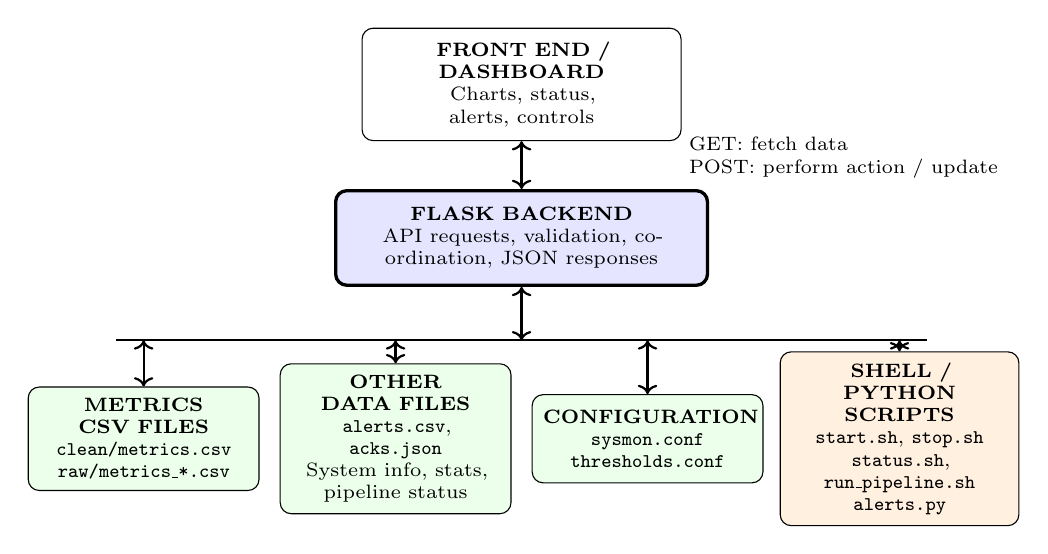
\begin{tikzpicture}[
  font=\scriptsize,
  front/.style={draw,rounded corners,fill=white,align=center,inner sep=5pt,
               text width=3.7cm,minimum height=0.75cm},
  backend/.style={draw,very thick,rounded corners,fill=blue!10,align=center,
                  inner sep=6pt,text width=4.3cm,minimum height=0.95cm},
  data/.style={draw,rounded corners,fill=green!8,align=center,inner sep=4pt,
              text width=2.65cm,minimum height=1.12cm},
  scripts/.style={draw,rounded corners,fill=orange!12,align=center,inner sep=4pt,
                  text width=2.75cm,minimum height=1.12cm},
  flow/.style={<->,thick},
  bus/.style={thick}
]

% Main layers
\node[front] (ui) at (0,2.95)
  {\textbf{FRONT END / DASHBOARD}\\Charts, status, alerts, controls};
\node[backend] (api) at (0,1.00)
  {\textbf{FLASK BACKEND}\\API requests, validation, coordination, JSON responses};

% Backend resources
\node[data] (metrics) at (-4.8,-1.55)
  {\textbf{METRICS CSV FILES}\\\texttt{clean/metrics.csv}\\\texttt{raw/metrics\_*.csv}};
\node[data] (other) at (-1.6,-1.55)
  {\textbf{OTHER DATA FILES}\\\texttt{alerts.csv}, \texttt{acks.json}\\System info, stats, pipeline status};
\node[data] (config) at (1.6,-1.55)
  {\textbf{CONFIGURATION}\\\texttt{sysmon.conf}\\\texttt{thresholds.conf}};
\node[scripts] (run) at (4.8,-1.55)
  {\textbf{SHELL / PYTHON SCRIPTS}\\\texttt{start.sh}, \texttt{stop.sh}\\\texttt{status.sh}, \texttt{run\_pipeline.sh}\\\texttt{alerts.py}};

% Front end requests and responses
\draw[flow] (ui.south) -- (api.north);
\node[align=left,anchor=west,fill=white,inner sep=2pt] at (2.05,2.02)
  {GET: fetch data\\POST: perform action / update};

% Shared resource bus and connections
\draw[flow] (api.south) -- (0,-0.30);
\draw[bus] (-5.15,-0.30) -- (5.15,-0.30);
\draw[flow] (-4.8,-0.30) -- (metrics.north);
\draw[flow] (-1.6,-0.30) -- (other.north);
\draw[flow] (1.6,-0.30) -- (config.north);
\draw[flow] (4.8,-0.30) -- (run.north);

\end{tikzpicture}

\vspace{2mm}
\footnotesize
Dashboard $\leftrightarrow$ backend: GET / POST.\\
Backend $\leftrightarrow$ files: read / update. \\
Backend $\rightarrow$ scripts: execute / collect result.
\end{frame}

\end{document}